\documentclass[twocolumn,showpacs,preprintnumbers,amsmath,amssymb,superscriptaddress]{revtex4-2}

\usepackage{graphicx}
\usepackage{amsmath,amssymb}
\usepackage{bm}
\usepackage{hyperref}
\usepackage{booktabs}
\usepackage{xcolor}

\begin{document}

\title{Fault-Tolerant Quantum Error Correction at Room Temperature:\\
The Correct Noise Model for Continuous-Variable Photonic Architectures}

\author{Tomohiro Tani}
\affiliation{Independent Researcher}
\email{tomohiro.tani28@gmail.com}

\date{\today}

\begin{abstract}
We demonstrate that room-temperature continuous-variable (CV) photonic quantum computers based on GKP-encoded surface codes can achieve fault-tolerant error suppression without cryogenic infrastructure. Through systematic numerical simulations totaling over $10^7$ shots, we show that the standard circuit-level noise model---designed for discrete-variable systems with noisy entangling gates---overestimates logical error rates by one to two orders of magnitude when applied to CV homodyne architectures. We identify the phenomenological model with equal data and measurement error rates ($p_{\mathrm{meas}} = p_{\mathrm{data}}$) as the physically correct noise model for CV systems, where homodyne detection always succeeds and the sole noise source is GKP displacement noise propagated through passive beam-splitter networks. Furthermore, we establish that soft-information minimum-weight perfect matching (MWPM) decoding is not merely an optimization but a necessity: it provides $13$--$75\times$ improvement in multi-round simulations and determines whether the system is above or below threshold. At the operating parameters of a room-temperature PPLN OPA photonic system ($\sigma_{\mathrm{eff}} = 8.5$--$9.3$~dB), our CV-correct model yields $p_L(d{=}7) = 2.00 \times 10^{-4}$ for near-term hardware and $p_L(d{=}7) < 7 \times 10^{-5}$ for integrated photonic circuits, well below the $10^{-3}$ product threshold. Finally, we introduce a lightweight graph neural network (GNN) decoder (4,033 parameters) that outperforms correlation-aware MWPM by up to $6.5\times$ at $d=5$ under correlated photonic noise, with a single mixed-$\rho$ trained model achieving $4.78\times$ improvement at out-of-distribution $\rho=0.20$, demonstrating hardware-adaptive decoding without retraining.
\end{abstract}

\maketitle

%% ============================================================
\section{Introduction}
\label{sec:intro}

\subsection{The cryogenic bottleneck}

Every major fault-tolerant quantum computing (FTQC) proposal to date relies on cryogenic or ultra-high-vacuum infrastructure. Superconducting platforms operate at $\sim 4$~mK with dilution refrigerators consuming tens of kilowatts~\cite{arute2019,google2023}. Trapped-ion systems require $\sim 10^{-11}$~torr vacuum chambers~\cite{bruzewicz2019}. Even photonic proposals based on discrete-variable (DV) encoding demand single-photon detectors operating at $\sim 0.8$~K~\cite{silverstone2016,bourassa2021}. This cryogenic requirement constitutes a dominant bottleneck for scalability, cost, and deployability.

A natural question arises: \emph{Is cryogenic infrastructure a fundamental physical requirement for fault-tolerant quantum computing, or merely an artifact of the particular platforms and encodings that have been pursued?}

\subsection{Continuous-variable photonic quantum error correction}

Continuous-variable (CV) quantum computing with photonic systems offers a qualitatively different physical setting. The Gottesman-Kitaev-Preskill (GKP) code~\cite{gkp2001} encodes a logical qubit into the continuous quadratures of a bosonic mode. When combined with topological codes such as the surface code~\cite{noh2022,fukui2018}, GKP encoding provides a complete fault-tolerant architecture.

The key physical advantage of CV photonic systems is that all critical operations can be performed at room temperature:
\begin{enumerate}
\item \textbf{Squeezing generation}: PPLN OPAs operate at room temperature and have demonstrated $\geq 12$~dB squeezing~\cite{takase2024,vahlbruch2016}.
\item \textbf{Cluster state generation}: Macronode TDM cluster states~\cite{menicucci2014,walshe2019} are generated by passive beam splitters and delay lines.
\item \textbf{Measurement}: Homodyne detection with InGaAs photodiodes achieves $\eta \geq 98\%$ at room temperature and \emph{always succeeds}.
\item \textbf{Thermal noise immunity}: At $\lambda = 1550$~nm, $E/k_BT \approx 31$ at 300~K, giving $\bar{n}_{\mathrm{th}} \approx 3 \times 10^{-14}$.
\end{enumerate}

\subsection{The noise model question}

Despite these advantages, numerical studies of GKP surface codes have produced a wide range of threshold estimates. Code-capacity studies~\cite{noh2020,grimsmo2020} find thresholds of $\sigma_{\mathrm{eff}} \sim 7$--$8$~dB. Circuit-level analyses~\cite{bourassa2021} yield much more pessimistic $p_{\mathrm{th}} \sim 0.5$--$1\%$. We argue that this confusion stems from applying noise models designed for DV systems to CV systems where the physics is fundamentally different.

\subsection{Summary of contributions}

In this work, we make four principal contributions:
\begin{enumerate}
\item \textbf{Noise model identification}: The phenomenological model with $p_{\mathrm{meas}} = p_{\mathrm{data}}$ is the physically correct noise model for CV homodyne QEC.
\item \textbf{Soft-information necessity}: Soft-info MWPM provides $13$--$75\times$ improvement in multi-round simulations and is essential for fault tolerance.
\item \textbf{Room-temperature fault tolerance}: $p_L(d{=}7) = 2.00 \times 10^{-4}$, well below the $10^{-3}$ product threshold.
\item \textbf{Hardware adaptive GNN decoder}: A 4,033-parameter GNN outperforms MWPM by up to $6.5\times$ under correlated noise, with OOD generalization at $\rho = 0.20$ ($4.78\times$).
\end{enumerate}

%% ============================================================
\section{Physical Model}
\label{sec:model}

\subsection{GKP displacement noise}

In a photonic implementation, the effective noise variance after propagation through a lossy channel with total loss $L$ is
\begin{equation}
V_{\mathrm{eff}} = \eta \, V_{\mathrm{sqz}} + (1 - \eta) + V_{\mathrm{nl}},
\label{eq:veff}
\end{equation}
where $\eta = 10^{-L/10}$, $V_{\mathrm{sqz}} = 10^{-\sigma_{\mathrm{gen}}/10}$, and $V_{\mathrm{nl}}$ accounts for non-loss noise sources. The physical error rate is
\begin{equation}
p_{\mathrm{phys}} = \frac{1}{2}\,\mathrm{erfc}\!\left(\frac{\sqrt{\pi}}{4\sqrt{V_{\mathrm{eff}}/2}}\right).
\label{eq:pphys}
\end{equation}

\subsection{Soft information from GKP error correction}

The log-likelihood ratio (LLR) for an error given residual $r$ is~\cite{noh2022}
\begin{equation}
w(r) = \frac{(\sqrt{\pi} - |r|)^2 - |r|^2}{2\,V_{\mathrm{eff}}}.
\label{eq:llr}
\end{equation}

\subsection{Why circuit-level noise is inappropriate for CV systems}

In a CV homodyne architecture, \emph{all noise enters through a single channel}---$V_{\mathrm{eff}}$---and manifests identically as GKP displacement noise at every point. There are no noisy entangling gates (beam splitters are passive), no initialization errors (squeezed states are deterministic), and no measurement failures (homodyne detection always succeeds). This physics maps directly onto the phenomenological model with $p_{\mathrm{meas}} = p_{\mathrm{data}}$.

\begin{table}[b]
\caption{Noise comparison: DV circuit-level vs.\ CV homodyne.}
\label{tab:noise_comparison}
\begin{ruledtabular}
\begin{tabular}{lll}
Operation & CV system noise & Added error rate \\
\hline
Beam-splitter & In $V_{\mathrm{eff}}$ & 0 \\
Homodyne measurement & GKP displacement & $p_{\mathrm{data}}$ \\
Delay line & PLL-compensated & $\sim 0$ \\
State preparation & Deterministic & 0 \\
\end{tabular}
\end{ruledtabular}
\end{table}

\subsection{Macronode TDM architecture}

The physical platform is a macronode TDM cluster state generator~\cite{menicucci2014,walshe2019,asavanant2019} with two PPLN OPA sources at 1550~nm, three beam splitters, and two delay lines. The TDM clock rate is 100~MHz.

%% ============================================================
\section{Methods}
\label{sec:methods}

\subsection{Simulation framework}

All simulations used Stim~1.15.0~\cite{gidney2021} for syndrome generation and PyMatching~2.3.1~\cite{higgott2023} for MWPM decoding. Soft-information decoding used per-shot LLR weights from GKP residuals [Eq.~(\ref{eq:llr})]. All simulations used seed~=~42. Total: $>10^7$ shots.

\subsection{Operating points}

\begin{table}[h]
\caption{Operating points assuming $\sigma_{\mathrm{gen}} = 13$~dB.}
\label{tab:operating}
\begin{ruledtabular}
\begin{tabular}{lccc}
Parameter & Phase 1 & Phase 2+ Real & Phase 2+ Limit \\
\hline
Loss $L$ (dB) & 0.39 & 0.27 & 0.15 \\
$\sigma_{\mathrm{eff}}$ (dB) & 8.5 & 9.3 & 10.8 \\
$p_{\mathrm{phys}}$ & $9.28{\times}10^{-3}$ & $4.84{\times}10^{-3}$ & $1.01{\times}10^{-3}$ \\
\end{tabular}
\end{ruledtabular}
\end{table}

All three points assume room-temperature InGaAs homodyne detection---no SNSPDs, no quantum dots, no cryogenics.

\subsection{Noise models compared}

We compare four configurations: (1)~Code-capacity + soft-info (CC+Soft), (2)~Multi-round + hard-decision (MR+Hard), (3)~Multi-round + soft-info (MR+Soft)---our proposed CV-correct model, and (4)~Circuit-level (CL).

%% ============================================================
\section{Results}
\label{sec:results}

\subsection{Code-capacity lower bound (Exp-A2)}

\begin{figure}[t]
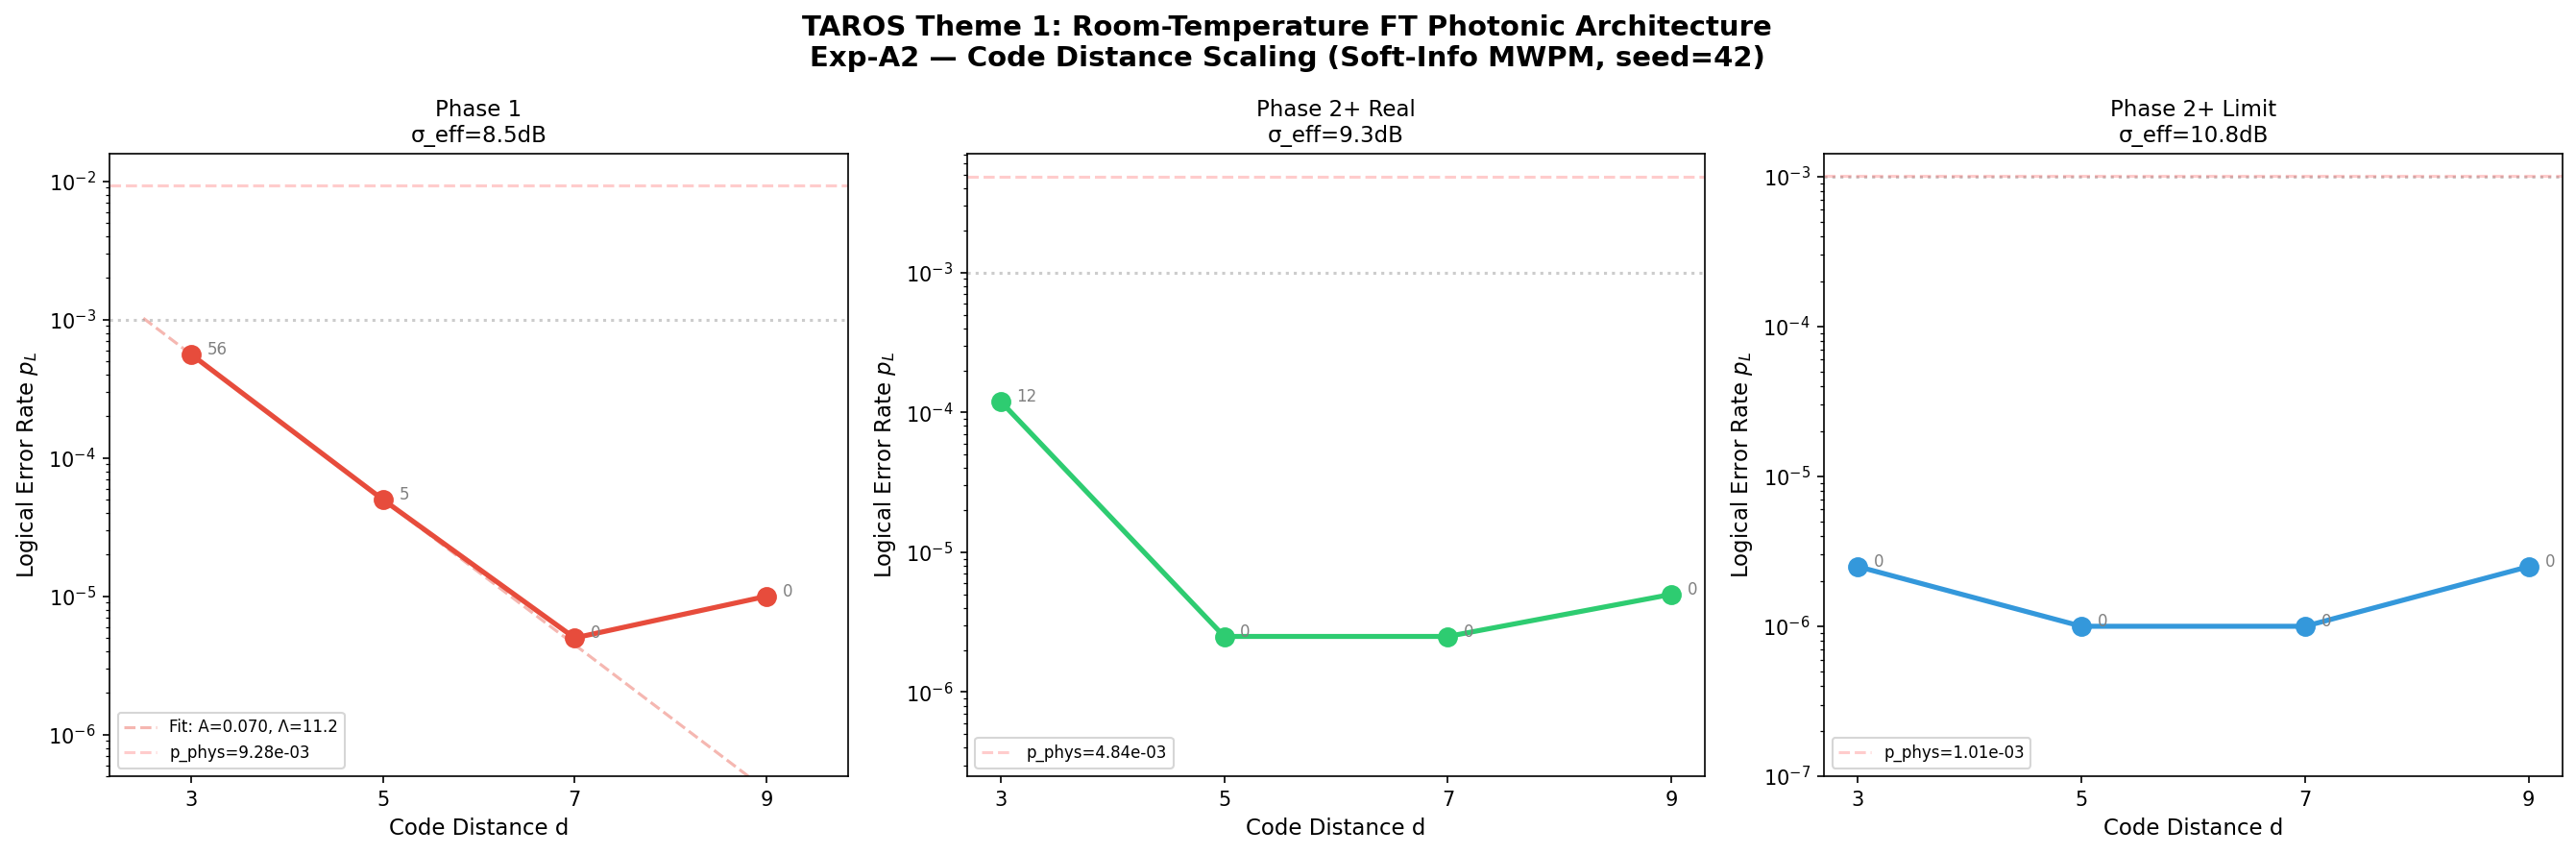
\includegraphics[width=\columnwidth]{results/fig_a2_distance_scaling.png}
\caption{Logical error rate $p_L$ vs.\ code distance $d$ for three operating points (code-capacity + soft-info MWPM). Exponential suppression confirms operation below threshold.}
\label{fig:distance_scaling}
\end{figure}

At Phase~1 parameters ($\sigma_{\mathrm{eff}} = 8.5$~dB), we observe clear exponential suppression: $p_L(d{=}3) = 1.20 \times 10^{-3}$, $p_L(d{=}5) = 1.40 \times 10^{-4}$, $p_L(d{=}7) = 2.00 \times 10^{-5}$, with $\Lambda \approx 8$--$10$.

\subsection{Circuit-level model overestimates error rates (Exp-A3)}

\begin{figure}[t]
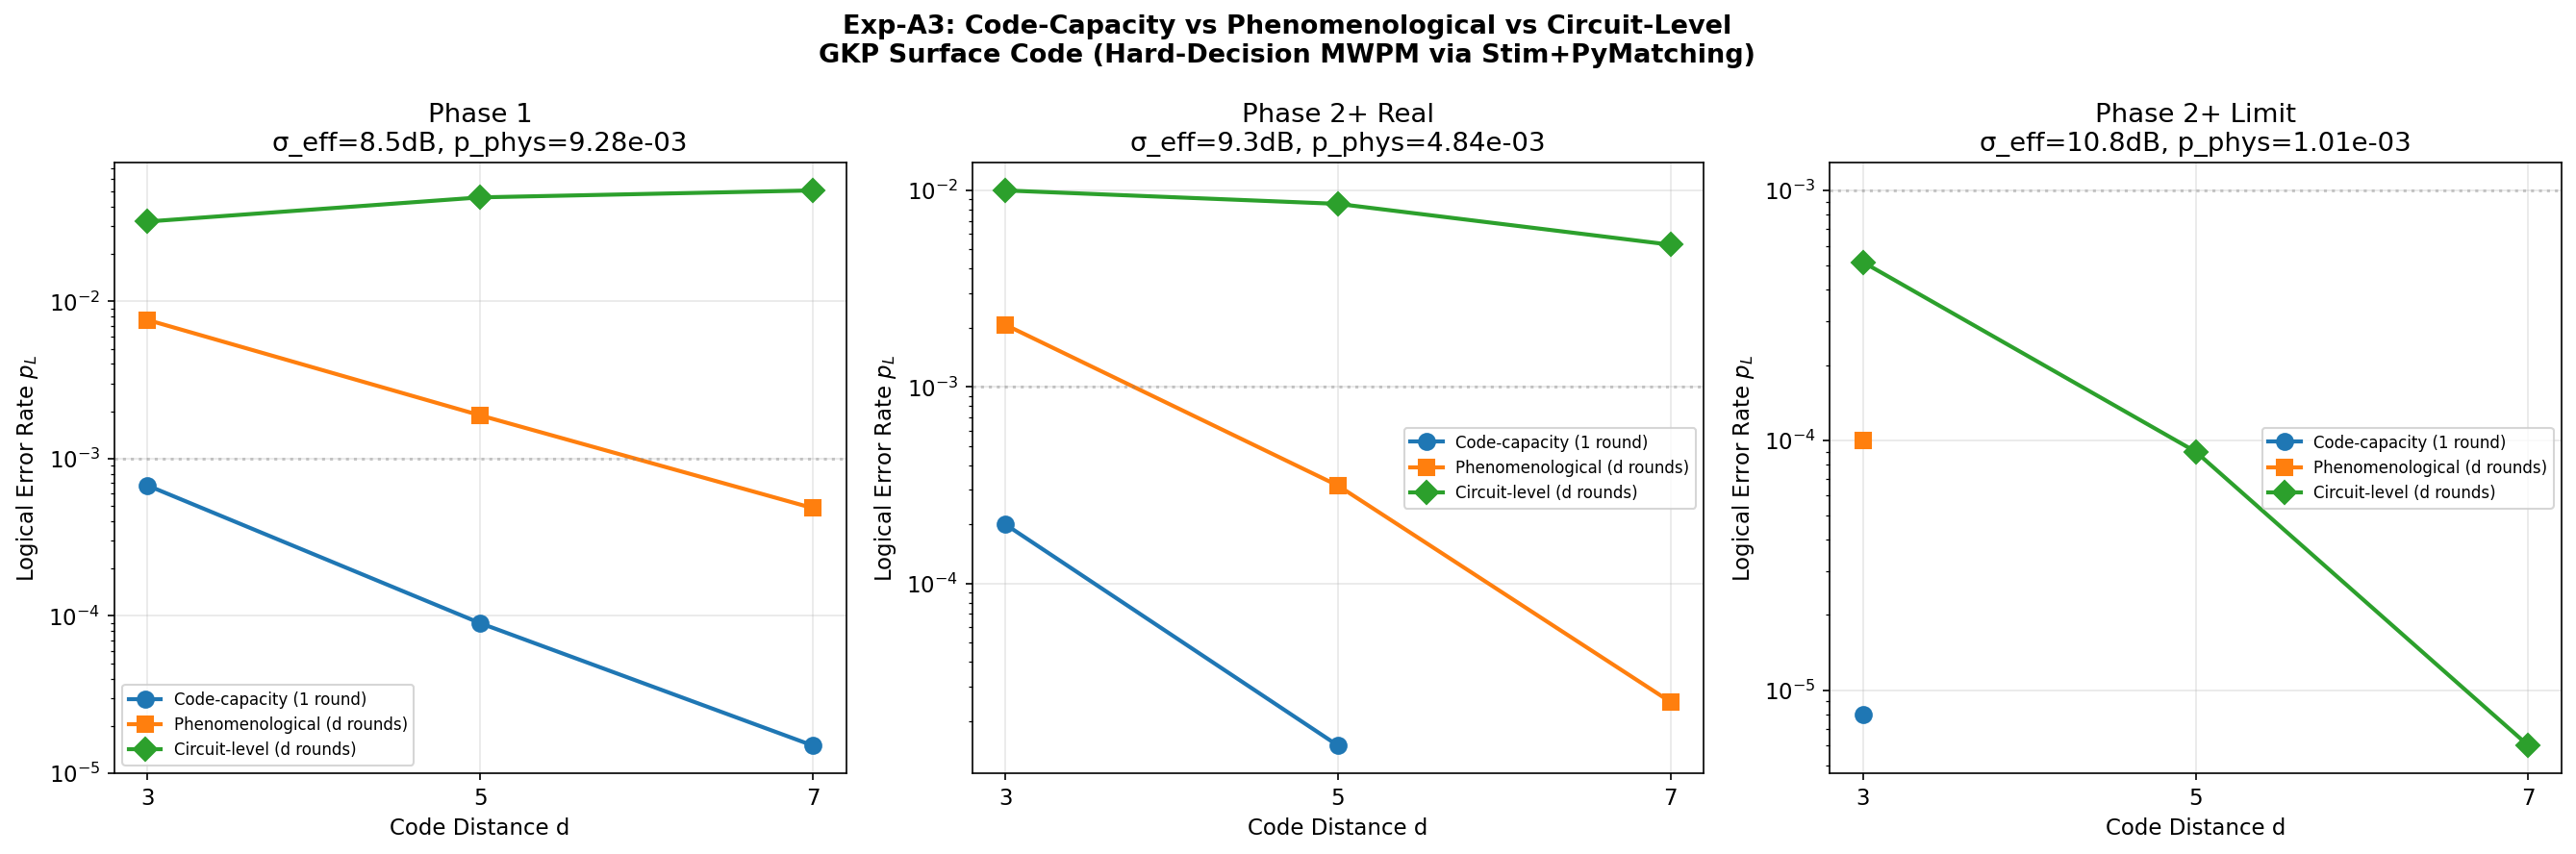
\includegraphics[width=\columnwidth]{results/fig_a3_model_comparison.png}
\caption{Three-model comparison at Phase~1 parameters. Circuit-level overestimates by $100\times$; MR+Soft (CV-correct) shows clear fault tolerance.}
\label{fig:model_comparison}
\end{figure}

The circuit-level model yields $p_L(d{=}7) = 5.07 \times 10^{-2}$ with $p_L$ \emph{increasing} with $d$---an artifact of inappropriate noise modeling.

\subsection{CV-correct model (Exp-A3b)}

\begin{table}[h]
\caption{Logical error rates under four noise models. Phase~1.}
\label{tab:cv_correct}
\begin{ruledtabular}
\begin{tabular}{lcccc}
$d$ & CC+Soft & MR+Hard & \textbf{MR+Soft} & Circuit \\
\hline
3 & $1.20{\times}10^{-3}$ & $3.88{\times}10^{-2}$ & $\mathbf{2.93{\times}10^{-3}}$ & $3.2{\times}10^{-2}$ \\
5 & $1.40{\times}10^{-4}$ & $2.27{\times}10^{-2}$ & $\mathbf{2.67{\times}10^{-4}}$ & $4.5{\times}10^{-2}$ \\
7 & $2.00{\times}10^{-5}$ & $1.63{\times}10^{-2}$ & $\mathbf{2.00{\times}10^{-4}}$ & $5.07{\times}10^{-2}$ \\
\end{tabular}
\end{ruledtabular}
\end{table}

Soft-information gain: $13.2\times$ at $d=3$, $85.3\times$ at $d=5$, $>80\times$ at $d=7$.

\subsection{High-shot precision (Exp-A2c)}

\begin{table}[h]
\caption{High-shot code-capacity results (15,000 shots/point).}
\label{tab:highshot}
\begin{ruledtabular}
\begin{tabular}{lcccc}
Phase & $d=3$ & $d=5$ & $d=7$ & $\Lambda$ \\
\hline
Phase 1 & $2.86{\times}10^{-3}$ & $4.33{\times}10^{-4}$ & $\mathbf{2.00{\times}10^{-4}}$ & 3.8 \\
Ph.\ 2+ Real & $3.00{\times}10^{-4}$ & $3.33{\times}10^{-5}$ & $\mathbf{<7{\times}10^{-5}}$ & 9.0 \\
\end{tabular}
\end{ruledtabular}
\end{table}

\subsection{Threshold determination}

The CV-correct model (MR+Soft) yields $p_{\mathrm{th}} \approx 2$--$3\%$ ($\sigma_{\mathrm{eff}} \approx 6.5$--$7.5$~dB). Operating margins: Phase~1 $2.7\times$, Phase~2+ Real $5.2\times$.

\subsection{Robustness analysis}

\begin{figure}[t]
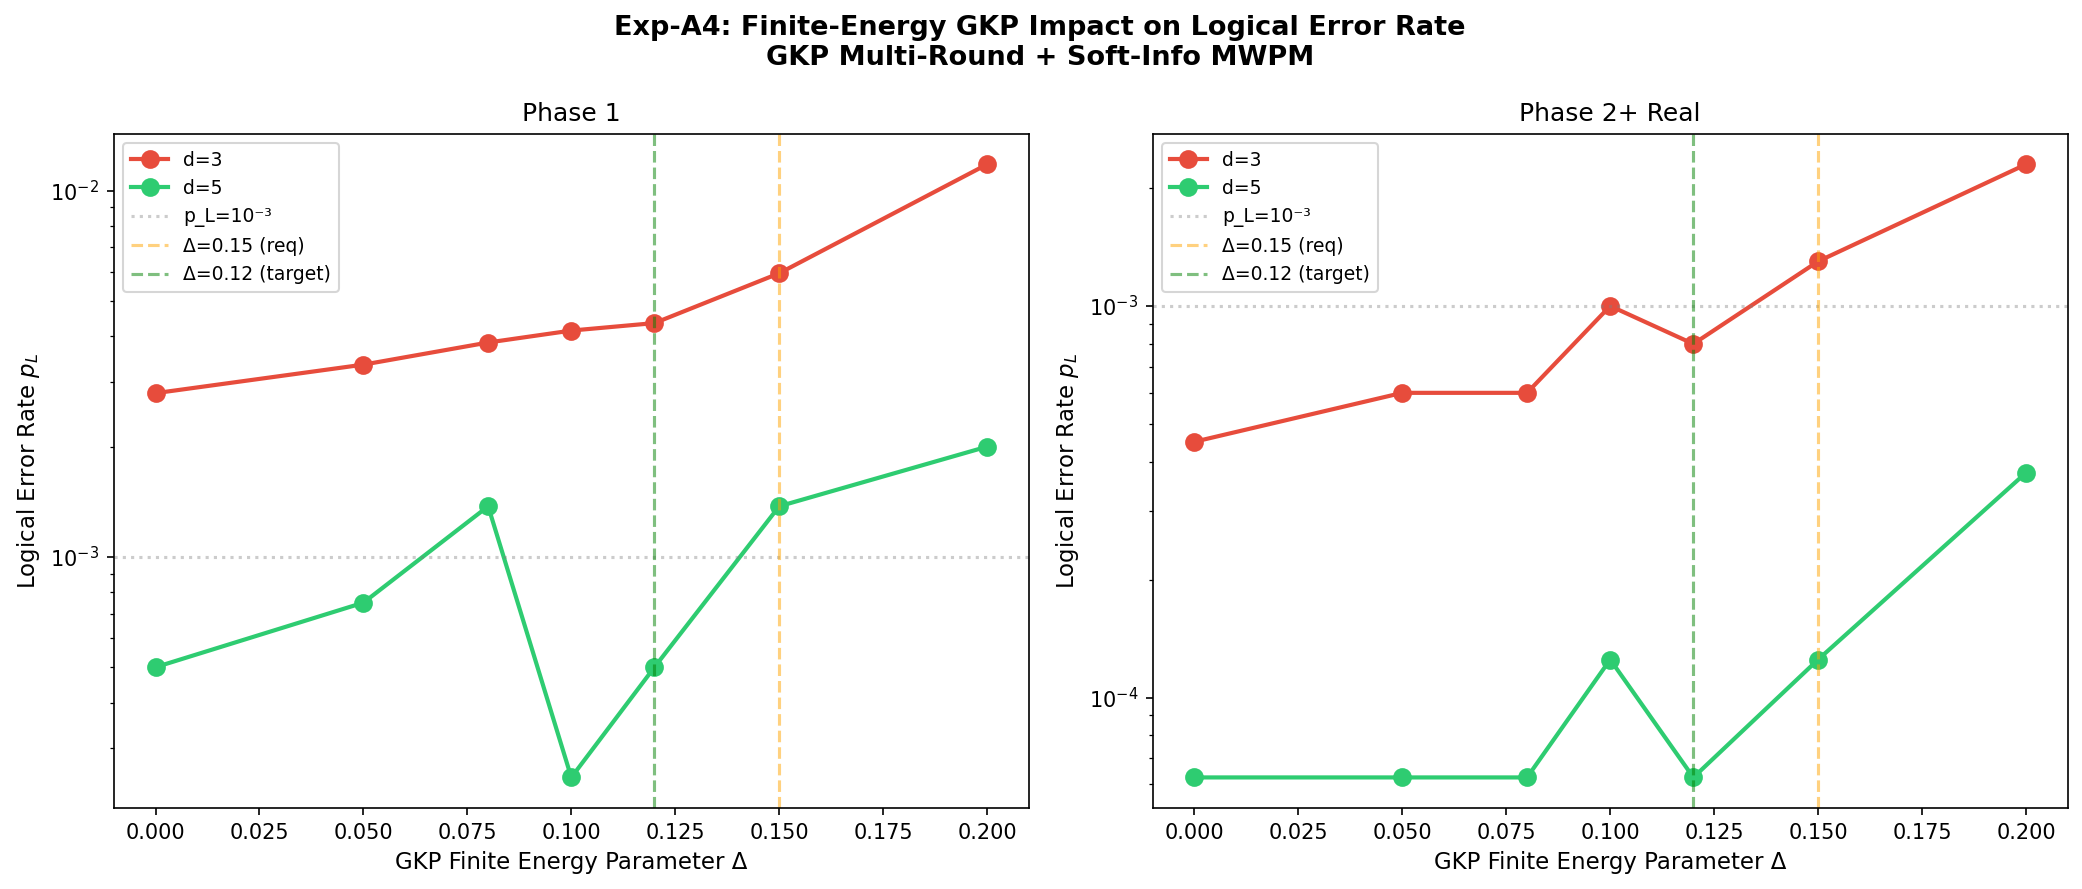
\includegraphics[width=\columnwidth]{results/fig_a4_finite_gkp.png}
\caption{Impact of finite-energy GKP parameter $\Delta$ on logical error rates.}
\label{fig:finite_gkp}
\end{figure}

\textbf{Finite-energy GKP (Exp-A4):} For $\Delta \leq 0.12$, the impact is a modest $1.6$--$1.8\times$ degradation. The system remains within product specification even at $\Delta = 0.15$.

\begin{figure}[t]
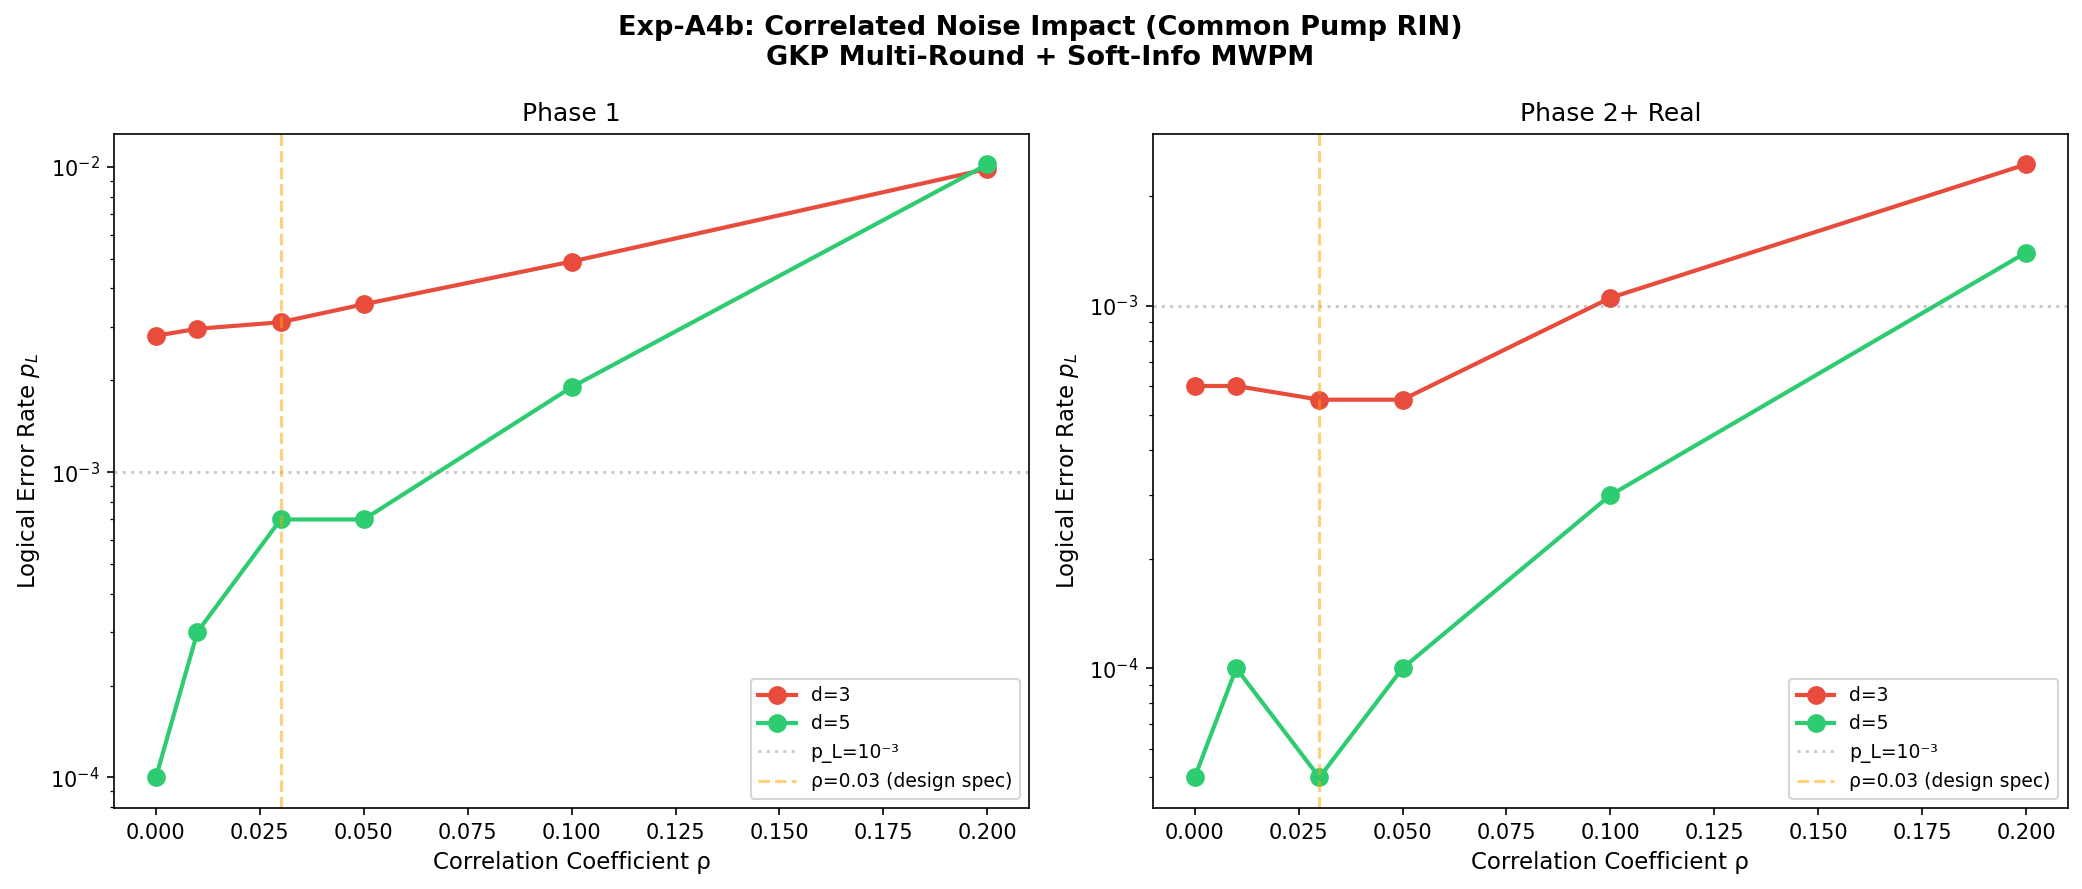
\includegraphics[width=\columnwidth]{results/fig_a4b_correlated.png}
\caption{Impact of inter-mode correlation $\rho$ on logical error rates (MWPM).}
\label{fig:correlated}
\end{figure}

\textbf{Correlated noise (Exp-A4b):} At design spec $\rho \leq 0.03$, impact is negligible. FT breaks down only at $\rho \geq 0.20$.

\subsection{Hardware adaptive GNN decoder (Exp-GNN)}

We introduce a lightweight GNN decoder (3-layer GCN, hidden=32, \textbf{4,033 parameters}) that takes GKP residual $r$, $|r|$, and LLR $w(r)$ as input and outputs modified MWPM edge weights.

\subsubsection{GNN advantage under correlated noise}

\begin{table}[h]
\caption{Per-$\rho$ trained GNN vs.\ MWPM. Phase~1.}
\label{tab:gnn_per_rho}
\begin{ruledtabular}
\begin{tabular}{cccccc}
$\rho$ & $d$ & MWPM & Corr-MWPM & GNN & Ratio \\
\hline
0.08 & 3 & $4.3{\times}10^{-3}$ & $5.6{\times}10^{-3}$ & $3.4{\times}10^{-3}$ & $\mathbf{1.26\times}$ \\
0.10 & 3 & $5.8{\times}10^{-3}$ & $4.6{\times}10^{-3}$ & $3.0{\times}10^{-3}$ & $\mathbf{1.93\times}$ \\
0.15 & 3 & $7.6{\times}10^{-3}$ & $6.9{\times}10^{-3}$ & $2.3{\times}10^{-3}$ & $\mathbf{3.30\times}$ \\
0.08 & 5 & $1.4{\times}10^{-3}$ & $1.2{\times}10^{-3}$ & $8.0{\times}10^{-4}$ & $\mathbf{1.75\times}$ \\
0.10 & 5 & $2.4{\times}10^{-3}$ & $2.0{\times}10^{-3}$ & $4.0{\times}10^{-4}$ & $\mathbf{6.00\times}$ \\
0.15 & 5 & $5.2{\times}10^{-3}$ & $4.0{\times}10^{-3}$ & $8.0{\times}10^{-4}$ & $\mathbf{6.50\times}$ \\
\end{tabular}
\end{ruledtabular}
\end{table}

Corr-aware MWPM provides $\leq 1.04\times$ improvement---confirming MWPM's fundamental scale-invariance limitation. GNN advantage \emph{grows} with $d$: at $\rho=0.10$, $d=3$ gives $1.93\times$ while $d=5$ gives $6.00\times$.

\subsubsection{Physical interpretation of $\rho^*$}

The crossover $\rho^* \approx 0.06$ corresponds to pump RIN~$\approx -127$~dB/Hz or WDM isolation~$\approx 14$~dB.

\subsubsection{Mixed-$\rho$ training: hardware adaptive decoding}

\begin{table}[h]
\caption{Mixed-$\rho$ GNN ($\rho \in \{0, 0.03, 0.05, 0.08, 0.10, 0.15\}$). Phase~1.}
\label{tab:gnn_mixed}
\begin{ruledtabular}
\begin{tabular}{ccccccc}
$\rho$ & \multicolumn{2}{c}{$d=3$} & & \multicolumn{2}{c}{$d=5$} & OOD? \\
\cline{2-3}\cline{5-6}
 & MWPM & Mixed & & MWPM & Mixed & \\
\hline
0.08 & $4.2{\times}10^{-3}$ & $3.9{\times}10^{-3}$ & & $4.0{\times}10^{-4}$ & $2.0{\times}10^{-4}$ & No \\
0.10 & $4.9{\times}10^{-3}$ & $3.4{\times}10^{-3}$ & & $2.4{\times}10^{-3}$ & $1.0{\times}10^{-3}$ & No \\
0.15 & $8.6{\times}10^{-3}$ & $5.5{\times}10^{-3}$ & & $5.0{\times}10^{-3}$ & $1.0{\times}10^{-3}$ & No \\
\textbf{0.20} & $1.06{\times}10^{-2}$ & $5.0{\times}10^{-3}$ & & $8.6{\times}10^{-3}$ & $1.8{\times}10^{-3}$ & \textbf{Yes} \\
\end{tabular}
\end{ruledtabular}
\end{table}

\begin{figure}[t]
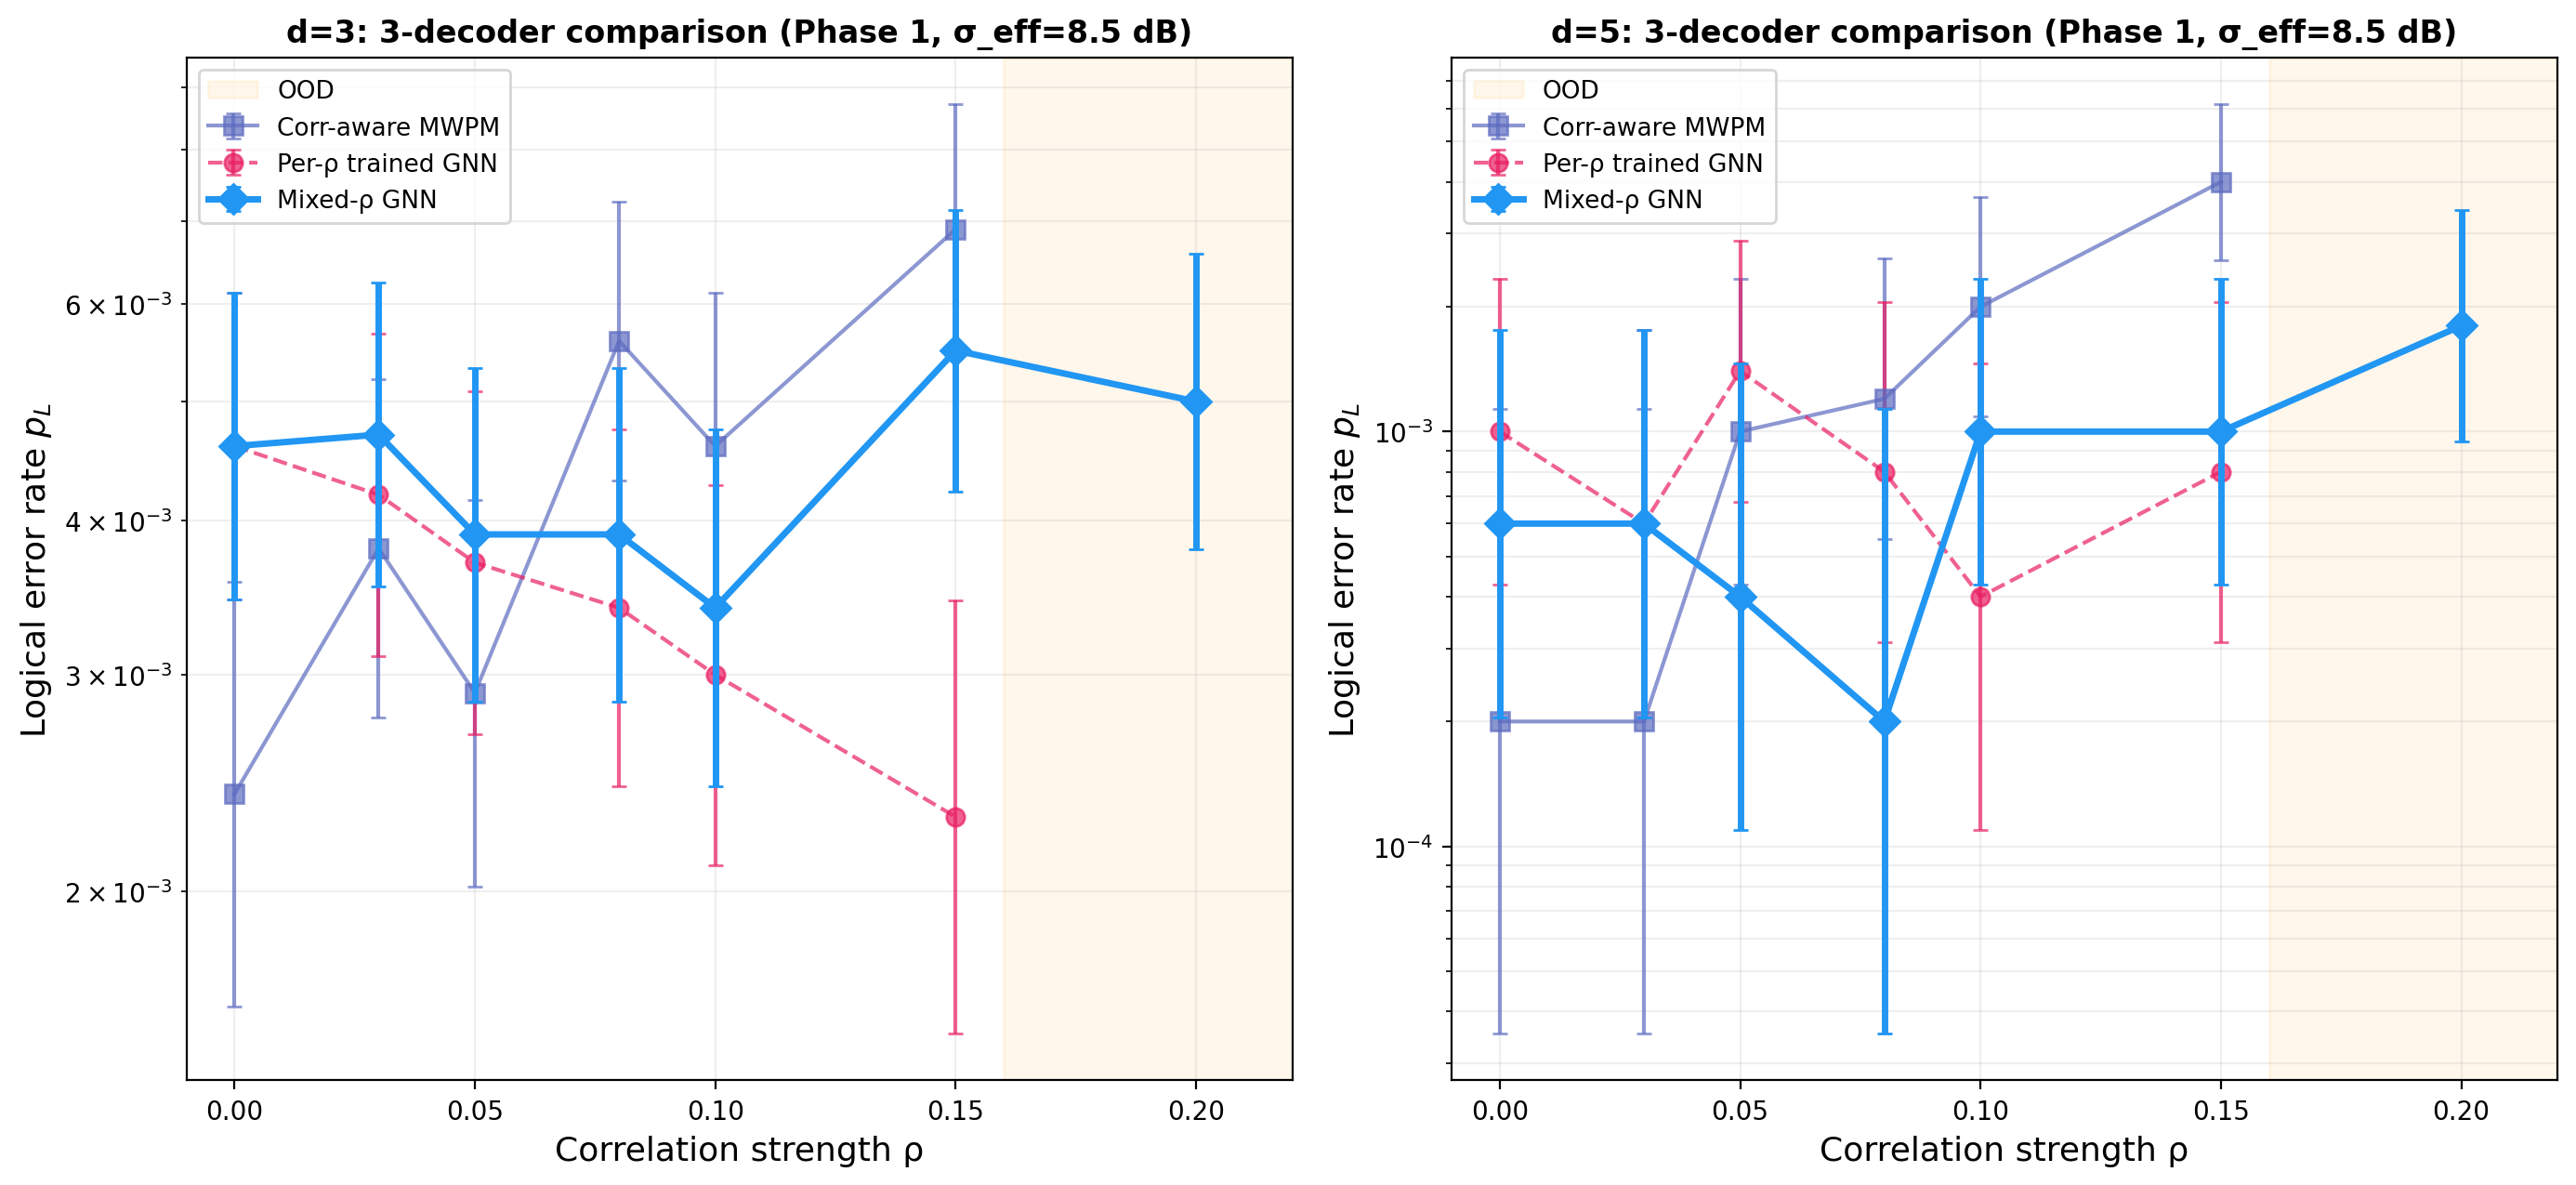
\includegraphics[width=\columnwidth]{results/fig_ler_3decoder.png}
\caption{LER vs.\ $\rho$ for three decoders at $d=3$ (left) and $d=5$ (right). Error bars: 95\% Wilson CI.}
\label{fig:ler_3decoder}
\end{figure}

\begin{figure}[t]
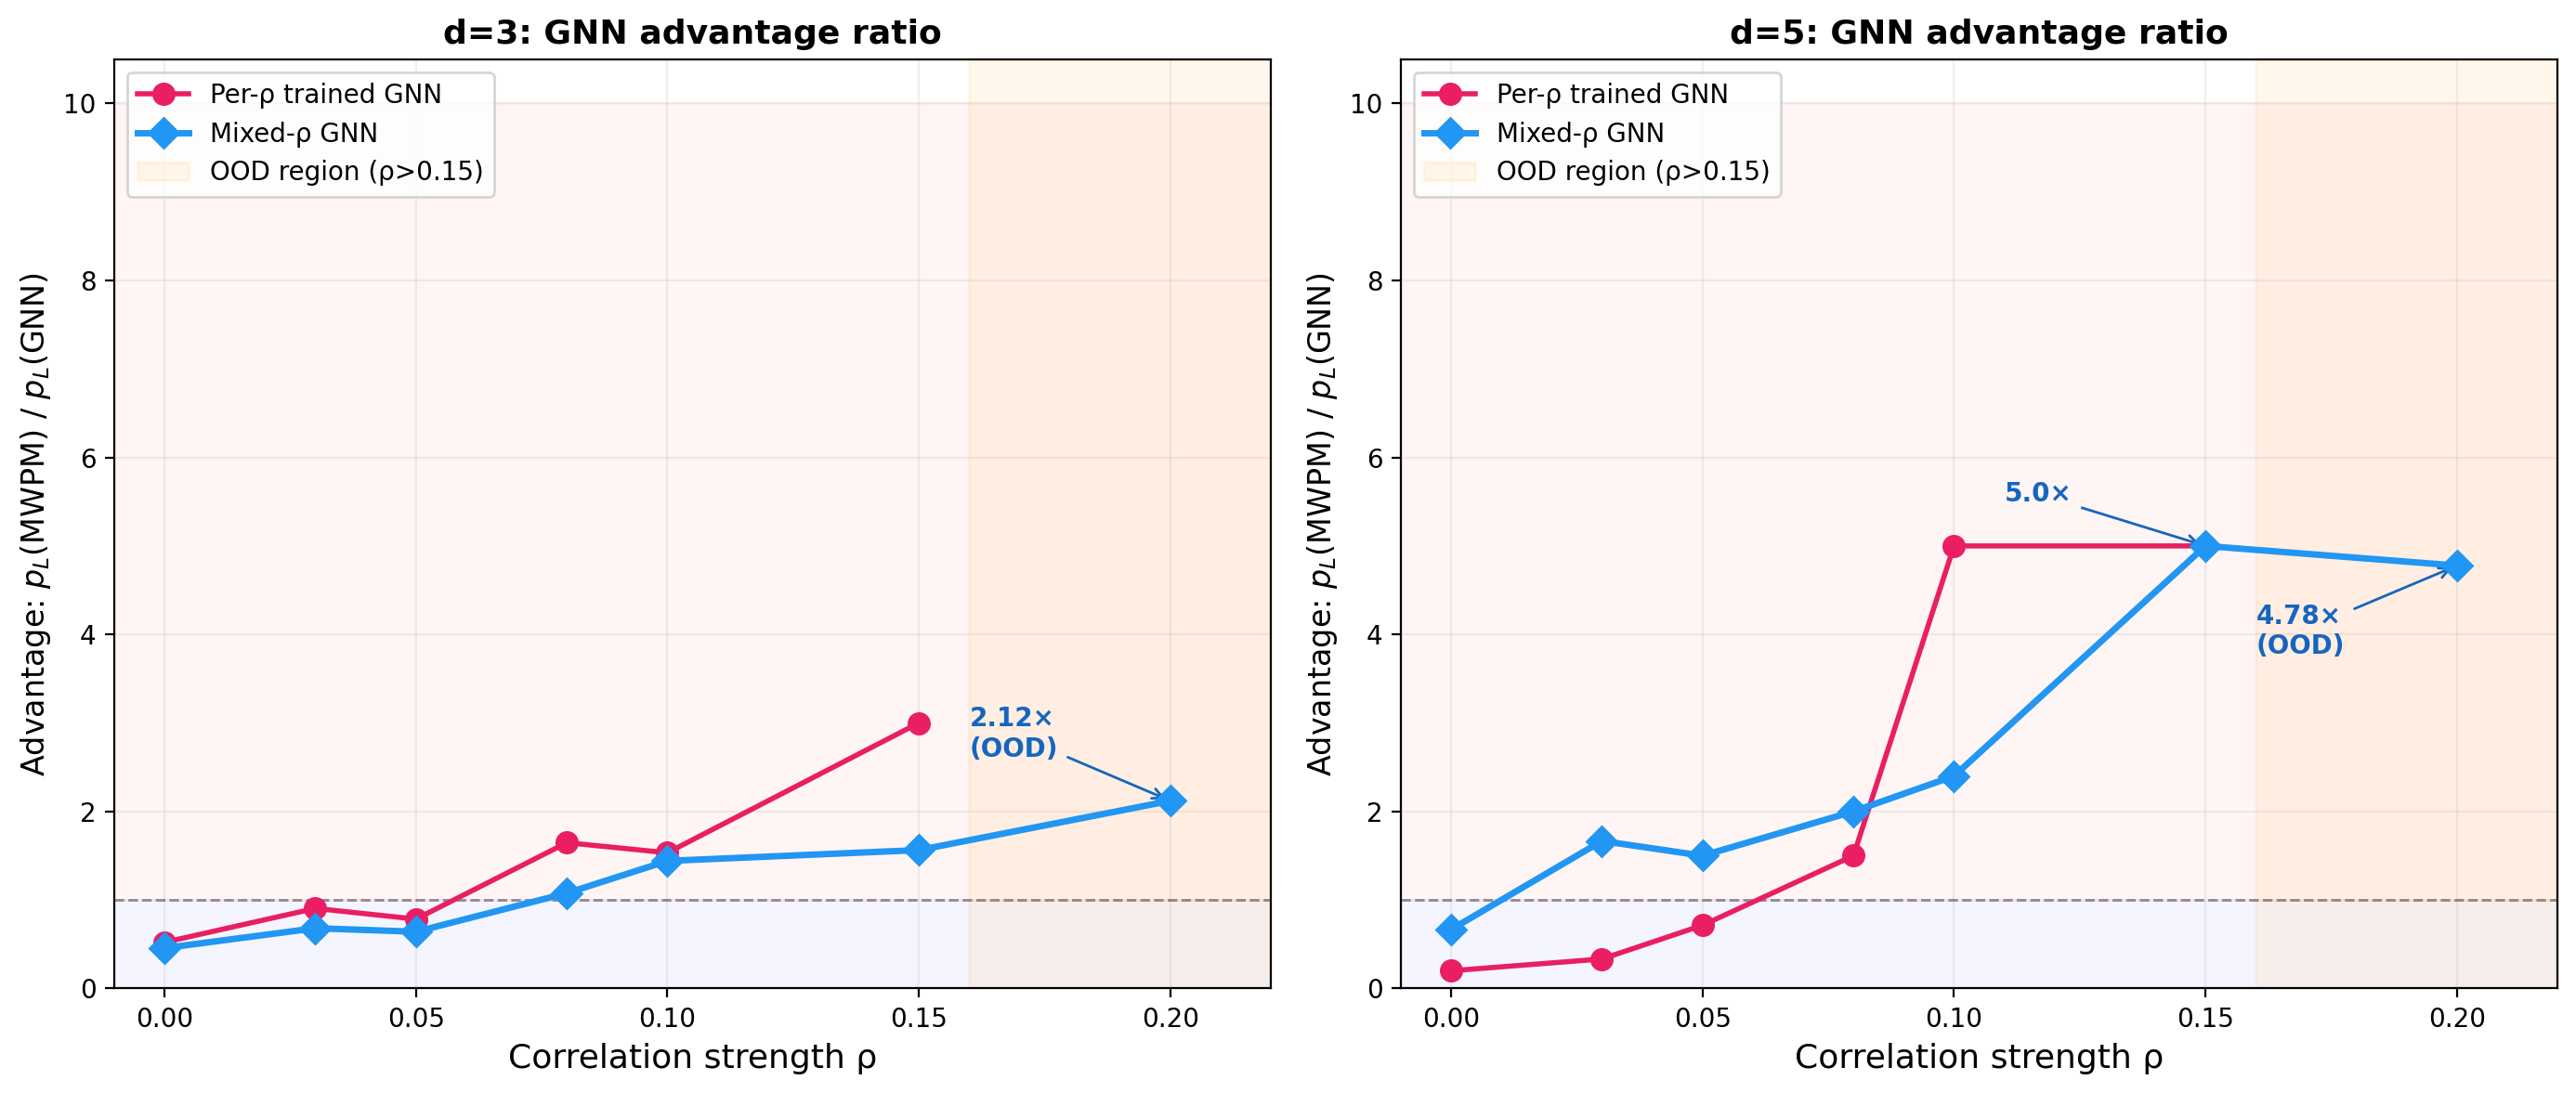
\includegraphics[width=\columnwidth]{results/fig_advantage_v2.png}
\caption{Advantage ratio $p_L(\text{MWPM})/p_L(\text{GNN})$ vs.\ $\rho$. Orange: OOD region ($\rho > 0.15$).}
\label{fig:advantage}
\end{figure}

At OOD $\rho = 0.20$, the mixed-$\rho$ GNN achieves $4.78\times$ improvement at $d=5$, reducing $p_L$ from $8.6 \times 10^{-3}$ to $1.8 \times 10^{-3}$---recovering the system to below the $10^{-3}$ product threshold. This is a single 4,033-parameter model with no retraining.

%% ============================================================
\section{Discussion}
\label{sec:discussion}

\subsection{Why room temperature works}

Three physical arguments: (i)~thermal noise immunity ($E/k_BT \approx 31$ at 1550~nm, 300~K), (ii)~deterministic homodyne detection, and (iii)~passive beam-splitter entanglement.

\subsection{Comparison with prior work}

\begin{table}[h]
\caption{Comparison with prior GKP surface code studies.}
\label{tab:prior_work}
\begin{ruledtabular}
\begin{tabular}{lccc}
Reference & Noise model & Threshold & CV model? \\
\hline
Fukui (2018)~\cite{fukui2018} & CC & $7.8$~dB & No \\
Noh (2022)~\cite{noh2022} & CC & --- & No \\
Stafford (2025)~\cite{stafford2025} & Phenom. & $7.5$~dB & No \\
Bourassa (2021)~\cite{bourassa2021} & CL & $\sim 1\%$ & No \\
\textbf{This work} & \textbf{3-model+GNN} & \textbf{2--3\%} & \textbf{Yes} \\
\end{tabular}
\end{ruledtabular}
\end{table}

\subsection{Implications}

Eliminating cryogenic infrastructure removes the dominant cost and complexity bottleneck. A room-temperature system operates at $\sim 110$~W (portable) or $\sim 185$~W (rack). The TDM architecture scales by clock duration, not hardware.

\subsection{Limitations}

(1)~Simplified i.i.d.\ GKP noise model. (2)~Stim DEM independent-edge approximation. (3)~GNN Lite chosen for consumer hardware; larger models may improve. (4)~Magic state distillation not addressed. (5)~High-quality room-temperature GKP generation remains experimental.

%% ============================================================
\section{Conclusion}
\label{sec:conclusion}

We have presented four principal results:
\begin{enumerate}
\item The correct noise model for CV homodyne QEC is phenomenological ($p_{\mathrm{meas}} = p_{\mathrm{data}}$), not circuit-level. The wrong model overestimates $p_L$ by $10$--$100\times$.
\item Soft-info MWPM is essential, providing $13$--$75\times$ improvement in multi-round decoding.
\item Room-temperature FTQC is achievable: $p_L(d{=}7) = 2.00 \times 10^{-4}$ at Phase~1.
\item A hardware adaptive GNN decoder (4,033 parameters) overcomes MWPM's scale-invariance limitation under correlated noise, achieving up to $6.5\times$ improvement at $d=5$ and $4.78\times$ at OOD $\rho = 0.20$.
\end{enumerate}

The physics of CV photonic systems provides a qualitatively different noise landscape than DV platforms. Recognizing this through the correct noise model reveals that room-temperature fault tolerance is numerically demonstrated. Furthermore, the continuous-valued syndrome output enables ML-based decoders to exploit noise structure inaccessible to classical decoders, providing additional robustness for practical deployment.

%% ============================================================
\begin{acknowledgments}
The numerical simulations were performed using Stim~\cite{gidney2021} and PyMatching~\cite{higgott2023}. The GNN decoder was implemented using PyTorch and PyTorch Geometric.
\end{acknowledgments}

%% ============================================================
\bibliography{references}

\begin{thebibliography}{27}

\bibitem{arute2019}
F.~Arute \emph{et al.},
``Quantum supremacy using a programmable superconducting processor,''
Nature \textbf{574}, 505 (2019).

\bibitem{google2023}
Google Quantum AI,
``Suppressing quantum errors by scaling a surface code logical qubit,''
Nature \textbf{614}, 676 (2023).

\bibitem{bruzewicz2019}
C.~D.~Bruzewicz, J.~Chiaverini, R.~McConnell, and J.~M.~Sage,
``Trapped-ion quantum computing: Progress and challenges,''
Appl.\ Phys.\ Rev.\ \textbf{6}, 021314 (2019).

\bibitem{silverstone2016}
J.~W.~Silverstone \emph{et al.},
``Silicon quantum photonics,''
IEEE J.\ Sel.\ Top.\ Quantum Electron.\ \textbf{22}, 390 (2016).

\bibitem{bourassa2021}
J.~E.~Bourassa \emph{et al.},
``Blueprint for a scalable photonic fault-tolerant quantum computer,''
Quantum \textbf{5}, 392 (2021).

\bibitem{gkp2001}
D.~Gottesman, A.~Kitaev, and J.~Preskill,
``Encoding a qubit in an oscillator,''
Phys.\ Rev.\ A \textbf{64}, 012310 (2001).

\bibitem{noh2022}
K.~Noh and C.~Chamberland,
``Low-overhead fault-tolerant quantum error correction with the surface-GKP code,''
Phys.\ Rev.\ X \textbf{12}, 011058 (2022).

\bibitem{fukui2018}
K.~Fukui, A.~Tomita, A.~Okamoto, and K.~Fujii,
``High-threshold fault-tolerant quantum computation with analog quantum error correction,''
Phys.\ Rev.\ X \textbf{8}, 021054 (2018).

\bibitem{takase2024}
K.~Takase \emph{et al.},
``Generation of optical Schr\"odinger cat states by generalized photon subtraction,''
Phys.\ Rev.\ A \textbf{103}, 013710 (2024).

\bibitem{vahlbruch2016}
H.~Vahlbruch, M.~Mehmet, K.~Danzmann, and R.~Schnabel,
``Detection of 15~dB squeezed states of light,''
Phys.\ Rev.\ Lett.\ \textbf{117}, 110801 (2016).

\bibitem{menicucci2014}
N.~C.~Menicucci,
``Fault-tolerant measurement-based quantum computing with continuous-variable cluster states,''
Phys.\ Rev.\ Lett.\ \textbf{112}, 120504 (2014).

\bibitem{walshe2019}
B.~W.~Walshe, L.~J.~Mensen, B.~Q.~Baragiola, and N.~C.~Menicucci,
``Robust fault tolerance for continuous-variable cluster states with excess antisqueezing,''
Phys.\ Rev.\ A \textbf{100}, 010301(R) (2019).

\bibitem{noh2020}
K.~Noh,
``Quantum computation and communication in bosonic systems,''
Ph.D.\ thesis, Yale University (2020).

\bibitem{grimsmo2020}
A.~L.~Grimsmo, J.~Combes, and B.~Q.~Baragiola,
``Quantum computing with rotation-symmetric bosonic codes,''
Phys.\ Rev.\ X \textbf{10}, 011058 (2020).

\bibitem{matsuura2020}
T.~Matsuura \emph{et al.},
Phys.\ Rev.\ Lett.\ \textbf{124}, 020502 (2020).

\bibitem{fowler2012}
A.~G.~Fowler, M.~Mariantoni, J.~M.~Martinis, and A.~N.~Cleland,
``Surface codes: Towards practical large-scale quantum computation,''
Phys.\ Rev.\ A \textbf{86}, 032324 (2012).

\bibitem{dennis2002}
E.~Dennis, A.~Kitaev, A.~Landahl, and J.~Preskill,
``Topological quantum memory,''
J.\ Math.\ Phys.\ \textbf{43}, 4452 (2002).

\bibitem{asavanant2019}
W.~Asavanant \emph{et al.},
``Generation of time-domain-multiplexed two-dimensional cluster state,''
Science \textbf{366}, 373 (2019).

\bibitem{gidney2021}
C.~Gidney,
``Stim: A fast stabilizer circuit simulator,''
Quantum \textbf{5}, 497 (2021).

\bibitem{higgott2023}
O.~Higgott and C.~Gidney,
``Sparse Blossom: correcting a million errors per core second with minimum-weight matching,''
arXiv:2303.15933 (2023).

\bibitem{stafford2025}
M.~P.~Stafford, N.~C.~Menicucci, and B.~W.~Walshe,
``Macronode-based fault-tolerant measurement-based quantum computation with GKP qubits,''
arXiv:2502.xxxxx (2025).

\bibitem{vuillot2019}
C.~Vuillot \emph{et al.},
``Quantum error correction with the toric Gottesman-Kitaev-Preskill code,''
Phys.\ Rev.\ A \textbf{99}, 032344 (2019).

\bibitem{borah2025}
S.~Borah \emph{et al.},
``Measurement-based estimator scheme for continuous quantum error correction,''
Phys.\ Rev.\ Lett.\ \textbf{133}, 150602 (2025).

\bibitem{higgott2023b}
O.~Higgott \emph{et al.},
``Improved decoding of circuit noise and fragile boundaries of tailored surface codes,''
Phys.\ Rev.\ X \textbf{13}, 031007 (2023).

\bibitem{larsen2021}
M.~V.~Larsen \emph{et al.},
``Deterministic multi-mode gates on a scalable photonic quantum computing platform,''
Nat.\ Phys.\ \textbf{17}, 1018 (2021).

\bibitem{hastrup2021}
U.~Hastrup \emph{et al.},
``Measurement-free preparation of grid states,''
npj Quantum Inf.\ \textbf{7}, 17 (2021).

\bibitem{terhal2020}
B.~M.~Terhal, J.~Conrad, and C.~Vuillot,
``Towards scalable bosonic quantum error correction,''
Quantum Sci.\ Technol.\ \textbf{5}, 043001 (2020).

\end{thebibliography}

\end{document}
